\chapter{ListBox View}
\label{sec:listbox_view}

A ListBox View displays DBContent data as text in tables to allow textual data inspection. When started, it presents itself in the following manner.

\begin{figure}[H]
    \hspace*{-2cm}
    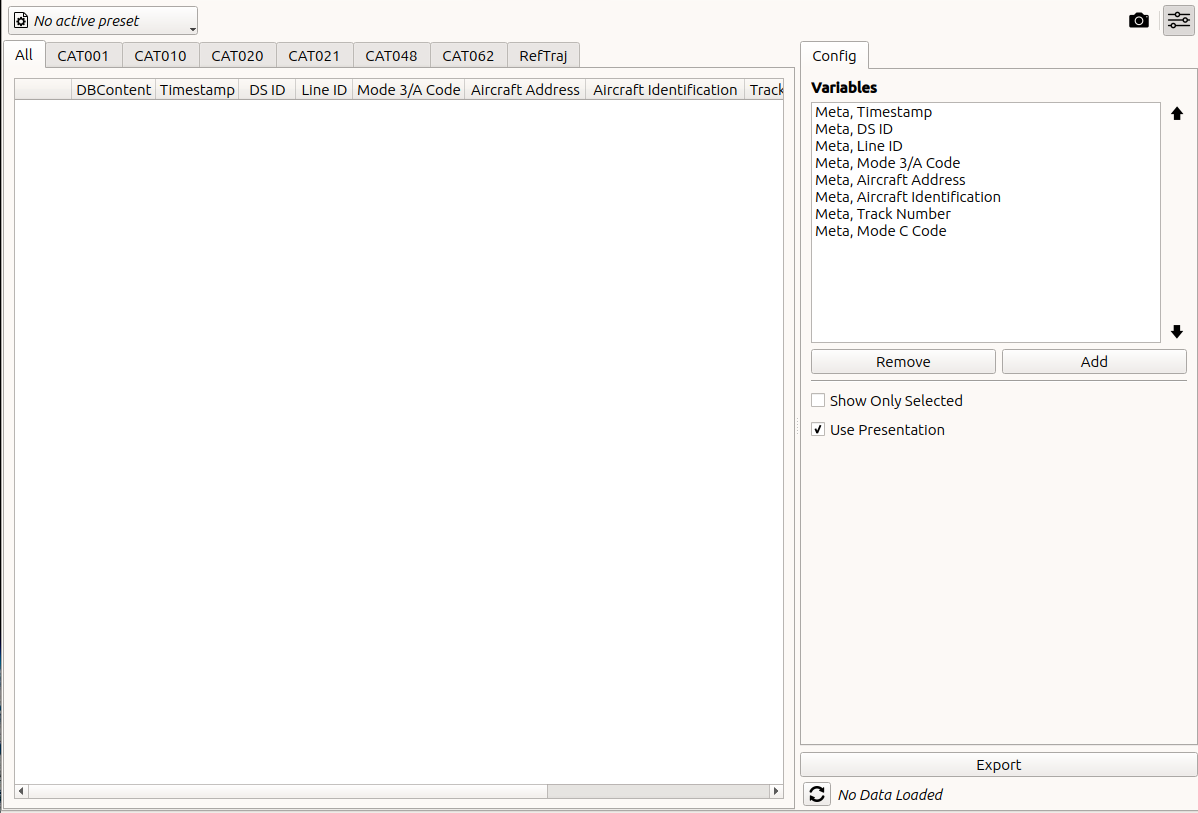
\includegraphics[width=18cm,frame]{figures/listbox_start.png}
  \caption{Listbox View startup}
  \label{fig:listbox_start}
\end{figure}

\section{Layout}

On the left side a number of tabs exist, one for each type of DBContent and an additional 'All' tab, each of which contains a table. \\

On the right side resides the configuration area, which allows configuring what data is loaded and how it is displayed.
The 
\includegraphics[width=0.5cm,frame]{../../data/icons/refresh.png} 'Reload' button on the bottom can be used to trigger a reload of the view's data.\\

Both areas can be resized and hidden if wanted.

\section{Data Loading}

To load the data the 'Reload' button or the mechanism described in Section \nameref{sec:ui_overview} can be used. To filter the dataset, the mechanism described in Section \nameref{sec:filters} can be used. \\

\begin{figure}[H]
    \hspace*{-2cm}
    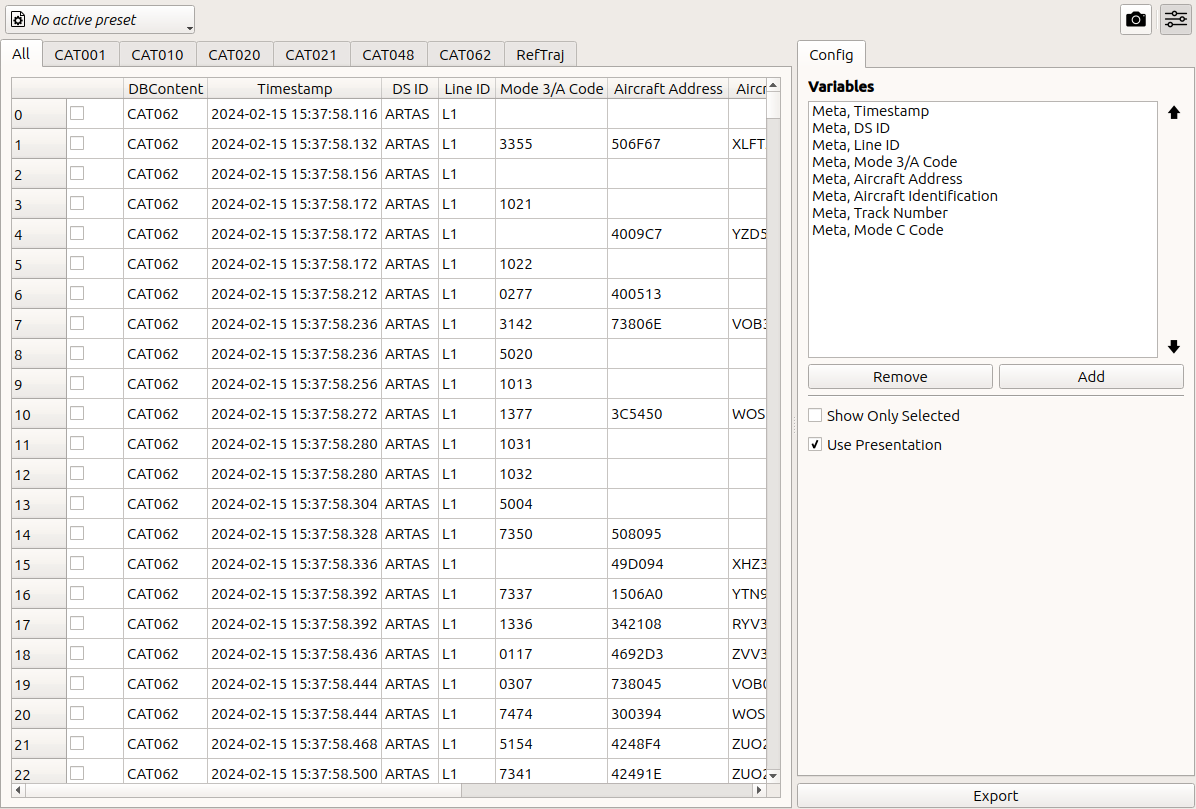
\includegraphics[width=18cm,frame]{figures/listbox_loaded.png}
  \caption{Listbox View after loading}
\end{figure}

Once updated, the tables are filled with text representing the values of the chosen DBContent variables. 
If a value is undefined its cell remains empy. For each type of DBContent a dedicated table is shown, as well as the 'All' table, where data from all DBContent types is shown collectively. \\

Please \textbf{note} that since a specific variable might only exist in certain DBContents, the number of columns in the various tables might differ.

\section{View Presets}

In the 'Variable Lists' section of the 'Config' tab, a variable list preset can be selected via a combo box. 
Further, custom variable lists can be added, copied and removed by the user. \\

The following presets exist:

%TODO_V7 Finalize variable lists
\begin{itemize}
\item Default: Common variables. Can not be renamed or removed.
\item Mode A/C Info: Includes the Mode A/C valid/garbled/smoothed flags.
\item Track Lifetime: Include the track begin/confirmed/coasted/end flags.
\item ADS-B Quality: Includes the ADS-B MOPS version, NACp/NUCp/NIC/SIL information.
\item Horizontal Movement: Includes horizontal movement modes and derivatives.
\item Vertical Movement: Includes vertical movement modes and derivatives.
\end{itemize}
\ \\

\section{Usage}

\subsection{Selection}

In the first column of each table checkboxes are shown, indicating whether that target report is currently selected. 
Selection may be changed by selecting/de-selecting the respective checkboxes, or by altering the selection in other views (cross-selection). 
If the selection is changed in one of the other views, this view is updated automatically.

\subsection{Variables}

For the selected variable list, all DBContent variables which are loaded from the database are shown in the 'Variables' list. 
This list is ordered, and like all configuration elements persistent. 
Ordering in the list can be changed by selecting a certain variable and using the up/down buttons to move it in the respective direction. \\

When pressing the 'Remove' button, a selected variable is removed. Pressing the 'Add' button allows appending a variable to the list using a context-menu. \\

If Meta variables are used, they are displayed for all DBContents they exist in. If a DBContent variable is used, it is only displayed in its native content.

\begin{figure}[H]
    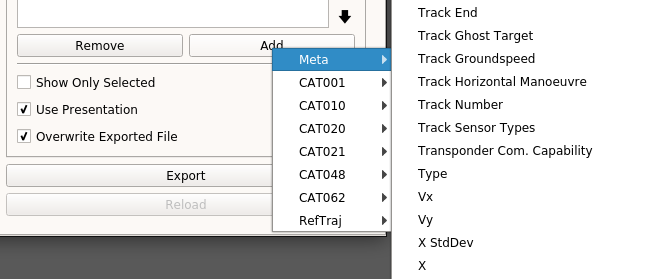
\includegraphics[width=16cm,frame]{figures/listbox_add.png}
  \caption{Listbox View adding of variables}
\end{figure}

After a adding a variable the dataset has to be reloaded to include the additional data, therefore the 'Reload' button becomes active.

\subsection{Show Only Selected}

%TODO_V7 Here the focus was on 'only selected in other views', but this actually has also effect on manual selection in this view?
When this checkbox is checked, only selected target reports are shown in the tables. In this mode, de-selecting a target report removes it from the shown data.

\subsection{Use Presentation}

When this checkbox is checked, the so called presentation mode is used. In the database, the variables might have different units or a data representations which is not easy to read. 
For this purpose, a presentation mode was introduced to e.g. show a Mode A code as octal, or a Time of Day not in seconds since midnight but in HH:MM:SS.SS format. \\

When the 'Use Presentation' checkbox is not checked, the original database values are presented (and exported).

%TODO Now solved via a metavariable, maybe remove in the future
%\subsection{Show Associations}
%When this checkbox is checked, the associated UTNs are shown for each target report. If no UTN is shown, this target reports was never associated to an UTN, 
%if several are shown (e.g. '1,2,4') this target report was used in several UTNs. \\
%This checkbox can only be used if association information is present in the database.

\subsection{Exporting}
\label{sec:exporting}

The data from the current  table can be exported to a comma-separated value (CSV) text, either as file or copied to the clipboard. \\

For this example a Mode 3/A code filter was used to load only target reports and system track updates from a single target. \\

To copy to the clipboard, select data to be copied in the table using the Shift key and the left mouse button, then press Ctrl-C. The CSV text data can then be pasted in other applications. \\

To export the complete loaded dataset, click the 'Export' button, so that a dialog is opened.

\begin{figure}[H]
    \hspace*{-2cm}
    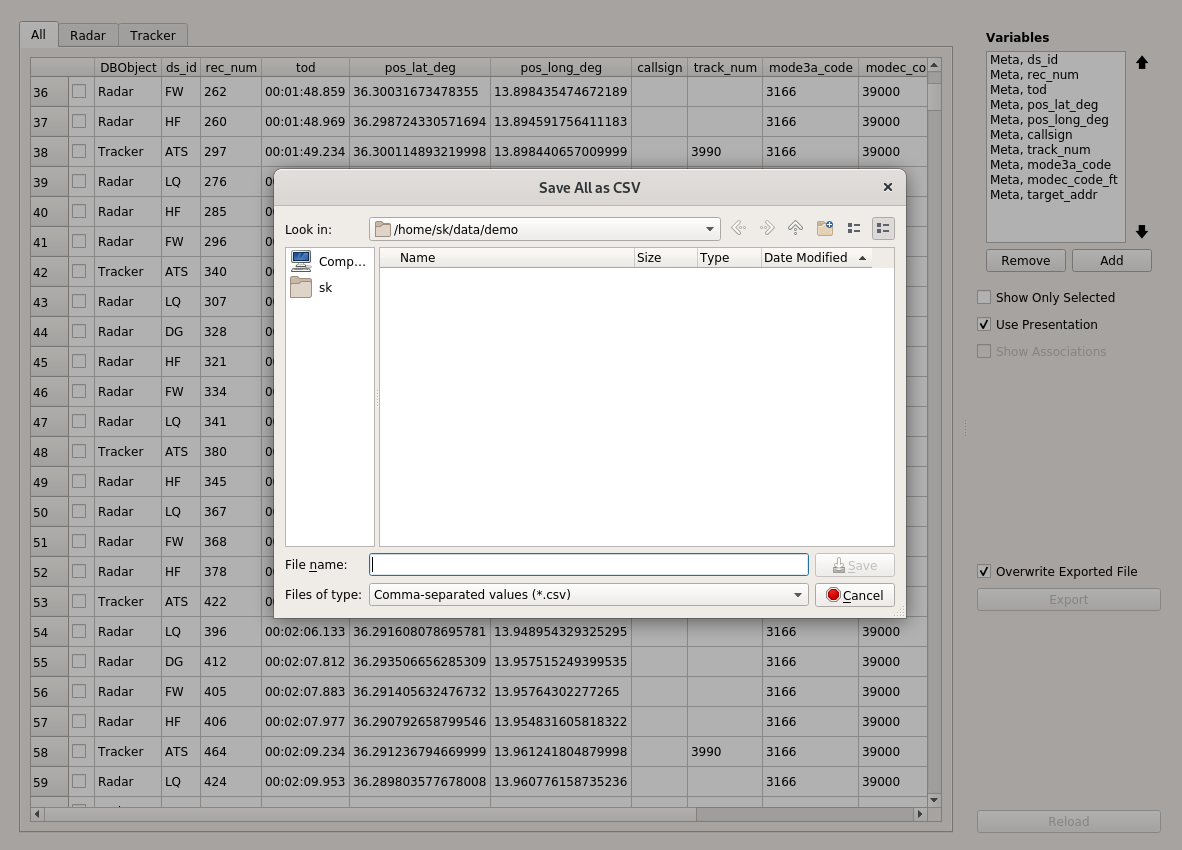
\includegraphics[width=18cm,frame]{figures/listbox_export.png}
  \caption{Listbox View export}
\end{figure}

Choose a filename, and press 'Save' to save the data. If the 'Overwrite Exported File' checkbox was checked, an existing file is automatically overwritten. Please \textbf{note} that exporting might take some time for larger datasets, and currently no status indication is given.\\

After export, a dialog is shown indicating that the export was completed. \\

The exported file can be opened in any editor, or for example imported into LibreOffice Calc.

\begin{figure}[H]
    \hspace*{-2.5cm}
    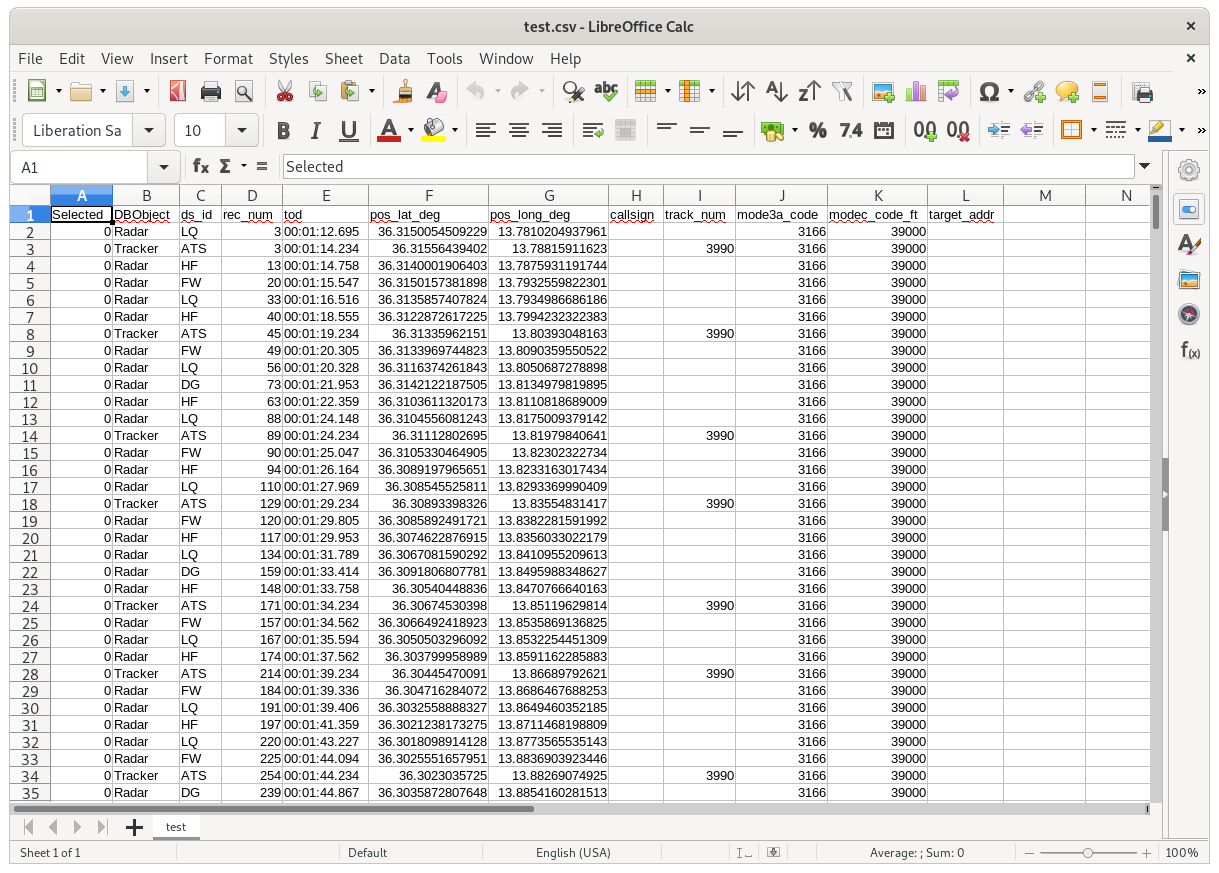
\includegraphics[width=19cm]{figures/listbox_exported_calc.png}
  \caption{Listbox View export in LibreOffice Calc}
\end{figure}
 
\subsection{Reload}

Additionally, if a change is made that requires re-loading of the data (e.g. additional data should be displayed) the 'Reload' button becomes available, and can be used to trigger a loading process. 
